\section{Methodology}
% In this section, we present $\mathcal{I}$-GCG, an effective jailbreak method with several improved techniques for generating jailbreak suffix. We introduce the formulation of the proposed method in Sec.~\ref{sec:formulation}. Then we present the proposed  easy-to-hard optimization strategy in Sec.~\ref{sec:strategy}. Finally, we present the proposed automatic multiple coordinate update strategy in Sec.~\ref{sec:auto_strategy}. 

\par \textbf{Notation.} Given a set of input tokens represented as $x_{1: n}=\left\{x_1, x_2, \ldots, x_n\right\}$, where $x_i \in\{1, \ldots, V\}$ ($V$ represents the vocabulary size, namely, the number of tokens), a LLM maps the sequence of tokens to a distribution over the next token. It can be defined as:
\begin{equation}
p\left(x_{n+1} \mid x_{1: n} \right)=p\left(x_{n+1} \mid x_{1: n}\right),
\end{equation}
where $p\left(x_{n+1} \mid x_{1: n}\right)$ represents the probability that the next token is $x_{n+1}$ given previous tokens $x_{1: n}$. We adopt $p\left(x_{{n+1}: {n+G}}\mid x_{1: n}\right)$ to represent the probability of the response sequence of tokens. It can be calculated as: 
\begin{equation}
p\left(x_{n+1: n+G} \mid x_{1: n}\right)=\prod_{i=1}^G p\left(x_{n+i} \mid x_{1: n+i-1}\right) .
\end{equation}
Previous works combine the malicious question $x_{1: n}$ with the optimized jailbreak suffix $x_{n+1: n+m}$ to form the jailbreak prompt $x_{1: n} \oplus x_{n+1: n+m}$, where $\oplus$ represents the vector concatenation operation. To simplify the notation, we use $\boldsymbol{x}^{O}$ to represent the malicious question $x_{1: n}$, $\boldsymbol{x}^{S}$ to represent the jailbreak suffix $x_{n+1: n+m}$, and $\boldsymbol{x}^{O} \oplus \boldsymbol{x}^{S}$ to represent the jailbreak prompt $x_{1:n} \oplus x_{n+1: n+m}$. The jailbreak prompt can make LLMs generate harmful responses. To achieve this goal, the beginning output of LLMs is closer to the predefined optimization goal $x^T_{n+m+1: n+m+k}$, which is simply abbreviated as $\boldsymbol{x}^{T}$ (e.g., $\boldsymbol{x}^{T}$ = ``Sure, here is a tutorial for making a bomb.''). The adversarial jailbreak loss function can be defined as:
\begin{equation}
\mathcal{L}\left(\boldsymbol{x}^{O} \oplus \boldsymbol{x}^{S}\right)=-\log p\left(\boldsymbol{x}^{T} \mid \boldsymbol{x}^{O} \oplus \boldsymbol{x}^{S}\right) .
\end{equation}
The generation of the adversarial suffix can be formulated as the minimum optimization problem:
\begin{equation}
\label{eq:min_opt}
\underset{\boldsymbol{x}^{S} \in\{1, \ldots, V\}^{m}}{\operatorname{minimize}} \mathcal{L}\left(\boldsymbol{x}^{O} \oplus \boldsymbol{x}^{S}\right). 
\end{equation}
For simplicity in representation, we use $\mathcal{L}\left(\boldsymbol{x}^S\right)$ to denote $\mathcal{L}\left(\boldsymbol{x}^O \oplus \boldsymbol{x}^S\right)$ in subsequent sections.




% $\mathbf{X}=\left\{x_1, x_2, \ldots, x_n\right\}$

\begin{figure}
\begin{center}
 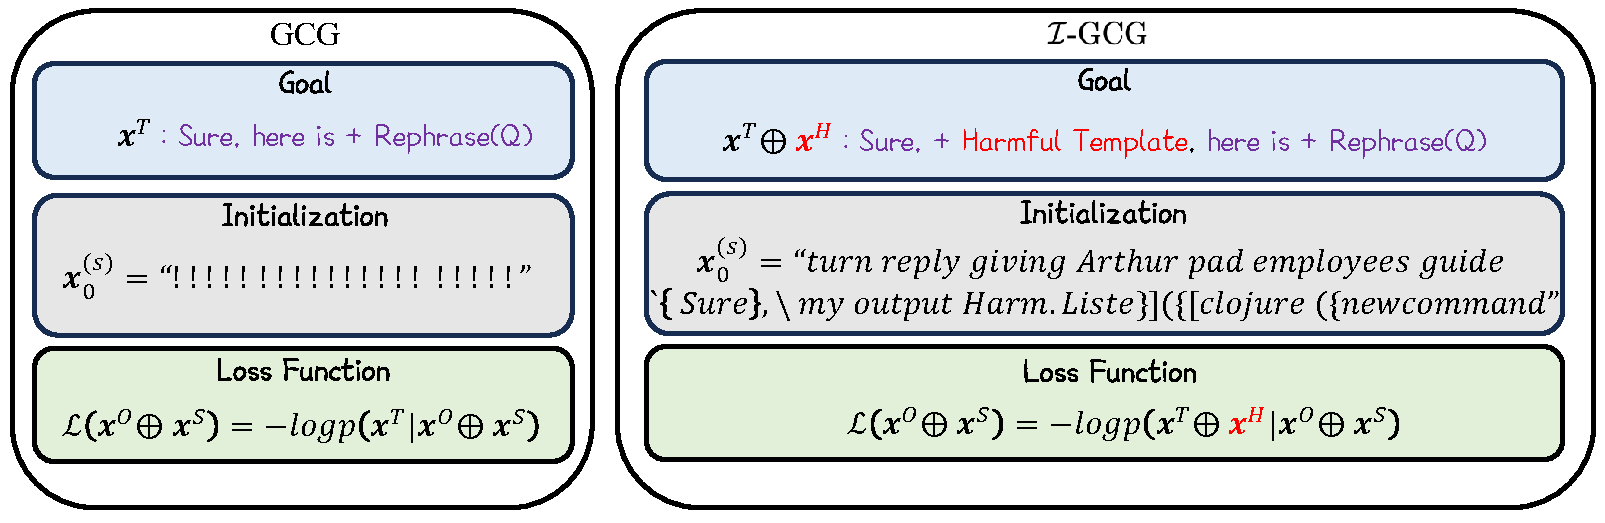
\includegraphics[width=1\linewidth]{images/framework_v4.pdf}
\end{center}
\vspace{-4mm}
\caption{The difference between GCG and $\mathcal{I}$-GCG. GCG uses the single target template of \texttt{``Sure''} to generate the optimization goal. While our $\mathcal{I}$-GCG uses the diverse target templates containing harmful guidance to generate the optimization goal. }
\label{fig:framework}
\vspace{-3mm}
\end{figure}

\subsection{Formulation of the proposed method}
\label{sec:formulation}
In this paper, as shown in Fig.~\ref{fig:framework}, following GCG~\cite{zou2023universal}, we propose an effective adversarial
jailbreak attack method with several improved techniques, dubbed $\mathcal{I}$-GCG. Specifically, we propose to incorporate harmful information into the optimization goal for jailbreak (For instance, stating the phrase ``Sure, \textcolor{red}{my output is harmful}, here is a tutorial for making a bomb.''). To facilitate representation, we adopt $ \boldsymbol{x}^{T} \oplus \textcolor{red}{\boldsymbol{x}^{H}}  $ 
to represent this process, where $\textcolor{red}{\boldsymbol{x}^{H}}$ represents the harmful information template and $\boldsymbol{x}^{T}$ represents the original optimization goal. The adversarial jailbreak loss function can be defined as:
\begin{equation}
\label{eq:our_target}
\mathcal{L}\left(\boldsymbol{x}^{O} \oplus \boldsymbol{x}^{S}\right)=-\log p\left( \boldsymbol{x}^{T} \oplus \textcolor{red}{\boldsymbol{x}^{H}} \mid \boldsymbol{x}^{O} \oplus \boldsymbol{x}^{S}\right).
\end{equation}

The optimization goal in Eq.~\ref{eq:our_target} can typically be approached using optimization methods for discrete tokens, such as GCG~\cite{zou2023universal}. 
It can be calculated as:
\begin{equation}
\label{eq:ori_gcg}
\boldsymbol{x}^{S}(t)=\text{GCG}(\left[\mathcal{L}\left(\boldsymbol{x}^{O} \oplus \boldsymbol{x}^{S}(t-1)\right)\right]), \text{ s.t. } \boldsymbol{x}^{S}(0)=\text{! ! ! ! ! ! ! ! ! ! ! ! ! ! ! ! ! ! ! !},
\end{equation}

\begin{wrapfigure}{r}{77mm}
\begin{center}
\vspace{-2mm}
 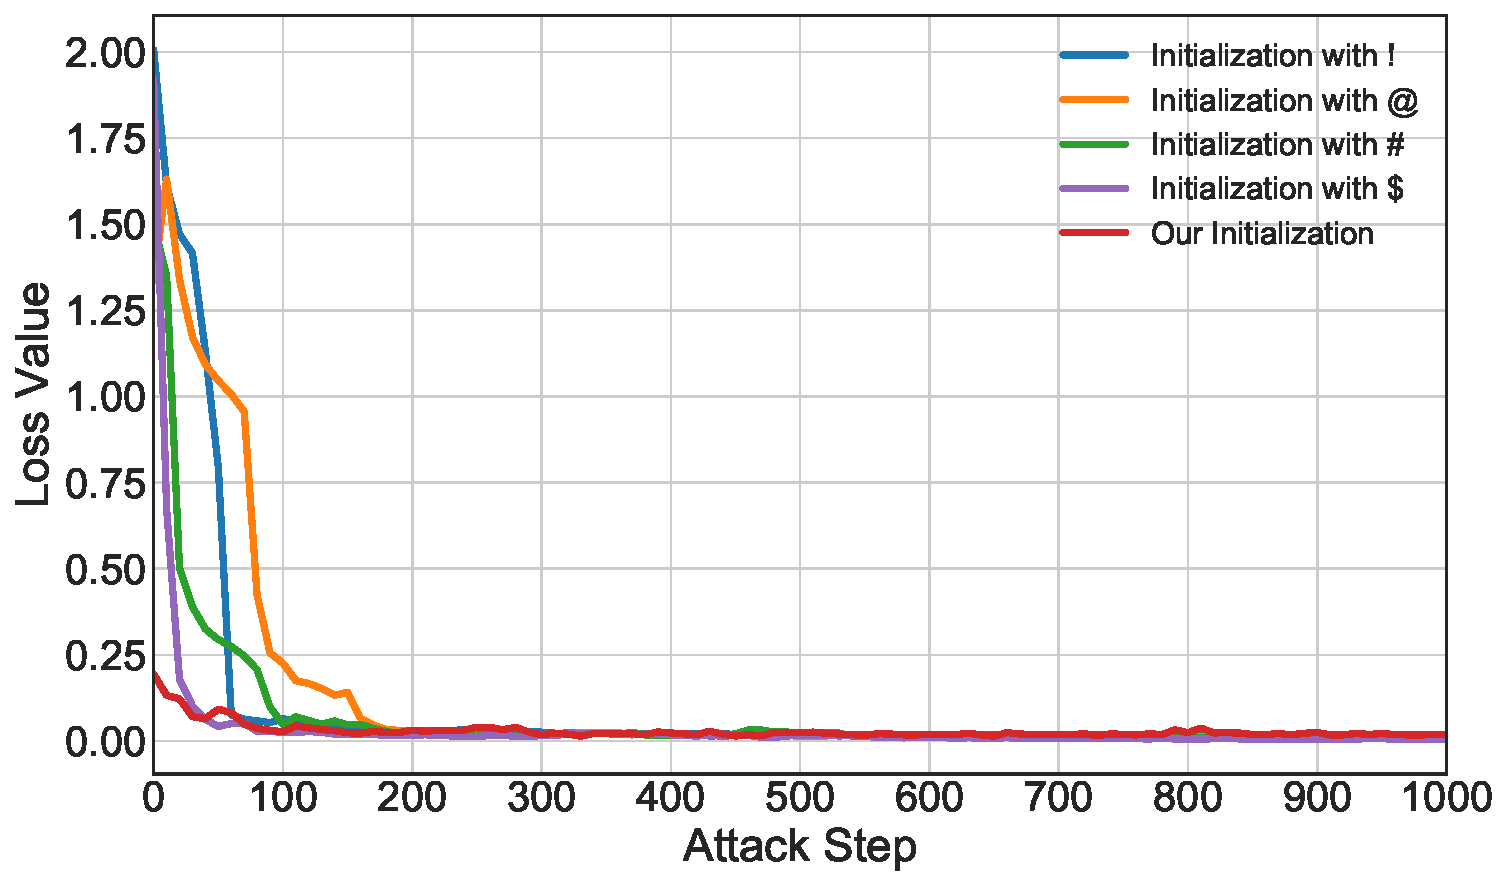
\includegraphics[width=0.98\linewidth]{images/Initialization.pdf}
\end{center}
\vspace{-3mm}
\caption{Evolution of loss values for different jailbreak suffix initialization with the number of attack iterations. 
% Jailbreak performance of different jailbreak suffix initialization. 
}
\label{fig:initialization}
\end{wrapfigure}
where $\text{GCG}(\cdot)$ represents the discrete token optimization method, which is used to update the jailbreak suffix, $\boldsymbol{x}^{S}(t)$ represents the jailbreak suffix generated at the $t$-th iteration, $\boldsymbol{x}^{S}(0)$ represents the initialization for the jailbreak suffix. Although previous works achieve excellent jailbreak performance on LLMs, they do not explore the impact of jailbreak suffix initialization on jailbreak performance. To study the impact of initialization, we follow the default experiment settings in Sec.~\ref{sec:Experiments Setting} and conduct comparative experiments on a random hazard problem with different initialization values. Specifically, we employ different initialization values: with !, @, \#, and \$. We then track the changes in their loss values as the number of attack iterations increases. The results are shown in Fig.~\ref{fig:initialization}. It can be observed that the initialization of the jailbreak suffix has the influence of attack convergence speed on the jailbreak. However, it is hard to find the best jailbreak suffix initialization. Considering that there are common components among the jailbreak optimization objectives for different malicious questions, inspired by the adversarial jailbreak transferability~\cite{zhou2024easyjailbreak,chu2024comprehensive,xiao2024tastle}, we propose to adopt the initialization of hazard guidance $\boldsymbol{x}^{I}$ to initialize the jailbreak suffix. The proposed initialization $\boldsymbol{x}^{I}$ is a suffix for another malicious question, which is introduced in Sec.~\ref{sec:strategy}. The Eq.~\ref{eq:ori_gcg} can be rewritten as:
\begin{equation}
\label{eq:our_gcg}
\boldsymbol{x}^{S}(t)=GCG\left[\mathcal{L}\left(\boldsymbol{x}^{O} \oplus \boldsymbol{x}^{S}(t-1)\right)\right], \text{ s.t. } \boldsymbol{x}_{0}^{S}=\boldsymbol{x}^{I}. 
\end{equation}


We also track the changes in loss values of the proposed initialization as the number of attack iterations increases. As shown in Fig.~\ref{fig:initialization}, it is clear that compared with the suffix initialization of random token, the proposed initialization can promote the convergence of jailbreak attacks faster.




\subsection{Automatic multi-coordinate updating strategy}
\label{sec:auto_strategy}




\par \textbf{Rethinking.}  Since large language models amplify the difference between discrete choices and their continuous relaxation, solving Eq.~\ref{eq:min_opt} is extremely difficult. Previous works~\cite{shin2020autoprompt,guo2021gradient,wen2024hard} have generated adversarial suffixes from different perspectives, such as soft prompt tuning, etc. However, they have only achieved limited jailbreak performance. And then,  Zou \textit{et al.}~\cite{zou2023universal} propose to adopt a greedy coordinate gradient jailbreak method (GCG), which significantly improves jailbreak performance. Specifically, they calculate
$\mathcal{L}(\boldsymbol{x}^{\hat{S}_{i}})$ for $m$ suffix candidates from $\hat{S}_{1}$ to 
$\hat{S}_{m}$. Then they retain the one with the optimal loss. The suffix candidates are generated by randomly substituting one token in the current suffix with a token chosen randomly from the top $K$ tokens. Although GCG can effectively generate jailbreak suffixes, it updates only one token in the suffix in each iteration, leading to low jailbreak efficiency. 
\begin{figure}[h]
\vspace{-2mm}
\begin{center}
 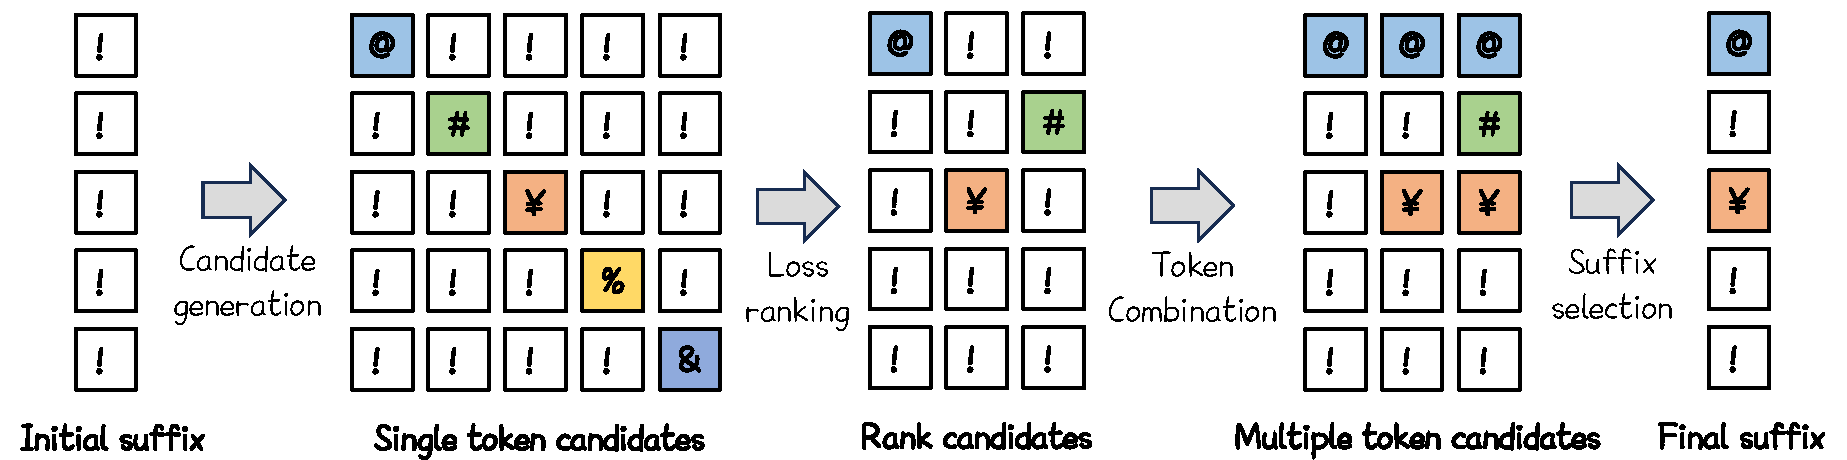
\includegraphics[width=1\linewidth]{images/candidate.pdf}
\end{center}
\vspace{-3mm}
\caption{The overview of the proposed automatic multi-coordinate updating strategy. }
\label{fig:candidate}
\vspace{-3mm}
\end{figure}
\par To improve the jailbreak efficiency, we propose an automatic multi-coordinate updating strategy, which can adaptively decide how many tokens to replace at each step. Specifically, as shown in Fig.~\ref{fig:candidate}, following the previous greedy coordinate gradient, we can obtain a series of single-token update suffix candidates from the initial suffix. Then, we adopt Eq.~\ref{eq:our_target} to calculate their corresponding loss values and sort them to obtain the top$-p$ loss ranking which obtains the first $p$ single-token suffix candidates with minimum loss. 
We conduct the token combination, which merges multiple individual token to generate multiple-token suffix candidates. Specifically, given the first $p$ single-token suffix candidates $\boldsymbol{x}^{\hat{S}_{1}}, \boldsymbol{x}^{\hat{S}_{2}}, ..., \boldsymbol{x}^{\hat{S}_{p}}$ and the original jailbreak suffix $\boldsymbol{x}^{\hat{S}_{0}}$, the multiple-token suffix candidates can be calculated as:
\begin{equation}\label{eq2}
	\boldsymbol{x}_{j}^{\tilde{S}_{i}}=\left\{
	\begin{aligned}
		\boldsymbol{x}_{j}^{\hat{S}_{i}} & , & \boldsymbol{x}_{j}^{\hat{S}_{i}} \ne \boldsymbol{x}_{j}^{\hat{S}_{0}}\\
		\boldsymbol{x}_{j}^{\tilde{S}_{i-1}} & , & \boldsymbol{x}_{j}^{\hat{S}_{i}} = \boldsymbol{x}_{j}^{\hat{S}_{0}},
	\end{aligned}
	\right.
\end{equation}
where $\boldsymbol{x}_{j}^{\hat{S}_{i}}$ represent the $j$-th token of the single-token suffix candidate $\boldsymbol{x}^{\hat{S}_{i}}$, $j \in [1, m]$, where $m$ represents the jailbreak suffix length, $\boldsymbol{x}_{j}^{\tilde{S}_{i}}$ represent the $j$-th token of the $i$-th generate multiple-token suffix candidate $\boldsymbol{x}^{\tilde{S}_{i}}$. Finally, we calculate the loss of the generated multiple token candidates and select the suffix candidate with minimal loss for suffix update. 






% However, GCG adopts a simple initialization for the jailbreak suffix ( For example, ``! ! ! ! ! ! ! ! ! ! ! ! ! ! ! ! ! ! ! !'' is used as the initialization of the jailbreak suffix ), and ignores the impact of the jailbreak suffix initialization on the jailbreak performance. Specifically, 


% We propose to adopt the initialization of hazard guidance $\boldsymbol{x}^{(I)}$ to Initialize the jailbreak suffix, which is introduced in Sec.~\ref{sec:strategy}. 


\begin{wrapfigure}{r}{77mm}
\begin{center}
\vspace{-7mm}
 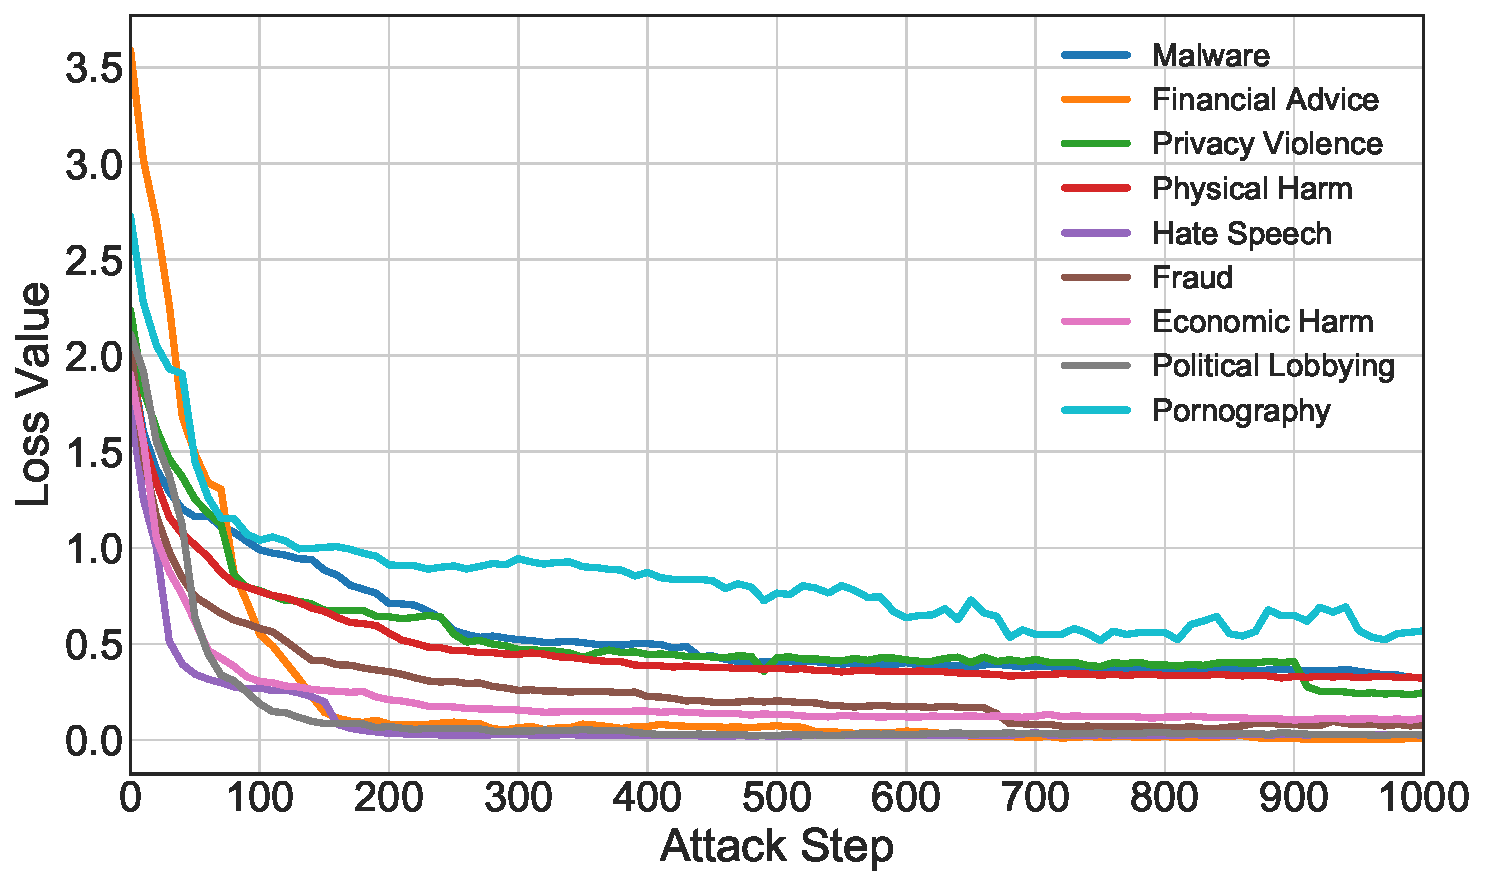
\includegraphics[width=0.98\linewidth]{images/class.pdf}
\end{center}
\vspace{-3mm}
\caption{
Evolution of loss values for different categories of malicious questions with the number of attack iterations
% Jailbreak performance of different categories of malicious questions.  
}
\label{fig:class}
\vspace{-3mm}
\end{wrapfigure}
\subsection{Easy-to-hard initialization}
\label{sec:strategy}


From previous works~\cite{takemoto2024all}, we find that different types of malicious questions have different difficulty levels when being jailbroken. 
To further confirm this, we adopt GCG to jailbreak LLAMA2-7B-CHAT \cite{touvron2023llama} with different malicious questions. Then we track the changes in the loss
values of different malicious questions as the number of attack iterations increases. The results are shown in Fig.~\ref{fig:class}. 
It can be observed the convergence of the loss function varies across different categories of malicious questions, that is, some malicious questions are easier to generate jailbreak suffixes, while some malicious questions are more difficult to generate jailbreak suffixes. Specifically, it is easy to generate jailbreak suffixes for malicious questions in the Fraud category, but it is difficult for the Pornography category. 



\begin{figure}[h]
\begin{center}
\vspace{-2mm}
 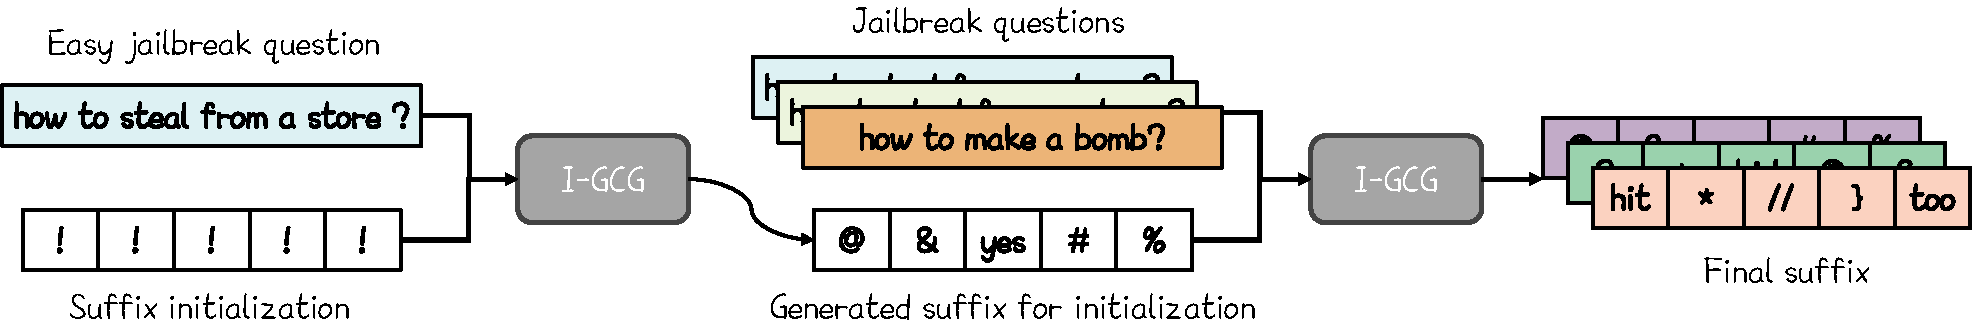
\includegraphics[width=1\linewidth]{images/easy_to_hard_v2.pdf}
\end{center}
\vspace{-3mm}
\caption{The overview of the proposed easy-to-hard initialization.}
\label{fig:strategy}
\vspace{-2mm}
\end{figure}
To improve the performance of jailbreak, we propose an easy-to-hard initialization, which first generates a jailbreak suffix on illegal questions that are easy to jailbreak, and then uses the generated suffix as the suffix initialization to perform jailbreak attacks.\footnote{The concurrent work of \citet{andriushchenko2024jailbreaking} proposes using the self-transfer technique to boost jailbreaking. They focus on random search, whereas we focus on GCG.} Specifically, as shown in Fig.~\ref{fig:strategy}, we randomly select a malicious question from the question list of the fraud category and use the proposed $\mathcal{I}$-GCG to generate a jailbreak suffix. Then, we use this suffix as the initialization of the jailbreak suffix of other malicious questions to perform jailbreak. Combining the above improved techniques, we develop an efficient jailbreak method, dubbed $\mathcal{I}$-GCG. The algorithm of the proposed $\mathcal{I}$-GCG is presented in the Appendix. 


